\documentclass[conference]{IEEEtran}
\IEEEoverridecommandlockouts
\usepackage{cite}
\usepackage{amsmath,amssymb,amsfonts}
\usepackage{algorithmic}
\usepackage{graphicx}
\usepackage{textcomp}
\usepackage{xcolor}
\usepackage{booktabs}
\usepackage{multirow}
\def\BibTeX{{\rm B\kern-.05em{\sc i\kern-.025em b}\kern-.08em
    T\kern-.1667em\lower.7ex\hbox{E}\kern-.125emX}}
\begin{document}

\title{Performance Evaluation of Post-Quantum Cryptographic Algorithms on C-V2X Sidelink Communications}

\author{
\IEEEauthorblockN{Akid Abrar}
\IEEEauthorblockA{\textit{Civil, Construction \& Environmental Eng.}\\
\textit{The University of Alabama}\\
Tuscaloosa, AL, USA\\
aabrar@ua.edu}
\and
\IEEEauthorblockN{Sagar Dasgupta}
\IEEEauthorblockA{\textit{Civil, Construction \& Environmental Eng.}\\
\textit{The University of Alabama}\\
Tuscaloosa, AL, USA\\
sdasgupta@ua.edu}
\and
\IEEEauthorblockN{Abdullah Al Mamun}
\IEEEauthorblockA{\textit{Civil Engineering}\\
\textit{Clemson University}\\
Clemson, SC, USA\\
abdullm@clemson.edu}
\and
\IEEEauthorblockN{Mizanur Rahman}
\IEEEauthorblockA{\textit{Civil, Construction \& Environmental Eng.}\\
\textit{The University of Alabama}\\
Tuscaloosa, AL, USA\\
mizan.rahman@ua.edu}
\and
\IEEEauthorblockN{Mashrur Chowdhury}
\IEEEauthorblockA{\textit{Civil Engineering}\\
\textit{Clemson University}\\
Clemson, SC, USA\\
mac@clemson.edu}
\and
\IEEEauthorblockN{Ahmad Alsharif}
\IEEEauthorblockA{\textit{Computer Science}\\
\textit{The University of Alabama}\\
Tuscaloosa, AL, USA\\
aalsharif1@ua.edu}
}

\maketitle

\begin{abstract}
The anticipated advent of quantum computing threatens current vehicular security standards based on elliptic curve cryptography. Post-quantum cryptographic (PQC) algorithms offer quantum resistance but introduce significantly larger signature and key sizes. This paper evaluates the National Institute of Standards and Technology (NIST) standardized Falcon-512 PQC digital signature scheme on Cellular-Vehicle-to-Everything (C-V2X) Mode~4 sidelink communications. This study evaluates the impact of Falcon-512's larger signature and public key size on sidelink key performance indicators, including packet delivery ratio (PDR), and end-to-end latency under moderate-high traffic density (30~veh/km). Results show that while Falcon-512 maintains comparable average latency (51.82~ms vs.\ 51.92~ms for ECDSA), the 470\% packet size overhead reduces mean PDR from 95.10\% to 71.18\%. These findings demonstrate that spectrum efficiency, rather than computational cost, is the primary bottleneck for PQC adoption in bandwidth-constrained V2X networks.
\end{abstract}

\begin{IEEEkeywords}
Post-quantum cryptography, C-V2X, Mode 4, sidelink, Falcon-512, performance evaluation
\end{IEEEkeywords}

\section{Introduction}

C-V2X communication enables vehicles to exchange safety-critical messages such as Basic Safety Messages (BSMs) via the PC5 Mode 4 sidelink interface without cellular infrastructure~\cite{3gpp_36213}. The IEEE~1609.2 standard specifies Elliptic Curve Digital Signature Algorithm (ECDSA) with the NIST P-256 curve for message authentication, producing 64-byte signatures and 65-byte public keys~\cite{ieee_16092}. However, Shor's algorithm can break elliptic curve cryptography using large-scale quantum computers~\cite{shor1994algorithms}, necessitating migration to post-quantum cryptographic alternatives.

The NIST has standardized lattice-based post-quantum signature schemes including FN-DSA (Falcon, FIPS~206)~\cite{fips206} and ML-DSA (Dilithium, FIPS~204)~\cite{fips204}. Falcon-512, the most compact NIST PQC scheme, produces signatures of approximately 666~bytes (padded) with 897-byte public keys, an order of magnitude larger than ECDSA. This payload inflation strains the C-V2X sidelink transport block constraints defined by SAE~J3161~\cite{sae_j3161}. The modulation and coding scheme (MCS) values between 5 and 11, 10 resource blocks (RB) subchannels, and 20 MHz channel bandwidth specified for the ITS 5.9 GHz band can accommodate a single Falcon-512 SPDU within one transport block (TB). But doing so consumes multiple subchannels per transmission and sharply increases total spectrum usage in dense traffic.


Prior studies have evaluated PQC computational overhead on embedded automotive hardware~\cite{kumar2024pqc_automotive} or analyzed protocol-layer integration~\cite{so2018pqc_protocols}, but have not quantified end-to-end sidelink performance under radio resource constraints. Post-quantum cryptography for vehicular networks has been explored primarily through computational benchmarking and protocol integration studies. Kumar et al.~\cite{kumar2024pqc_automotive} evaluated PQC signing and verification latency on automotive-grade processors, demonstrating sub-5~ms latency for Falcon-512, well within safety application requirements. So and Ma~\cite{so2018pqc_protocols} analyzed PQC integration into IEEE~1609.2 certificate provisioning but did not evaluate radio resource impact. Lee et al.~\cite{lee2025pqc_ami} recently assessed PQC feasibility for Advanced Metering Infrastructure using QEMU-based hardware emulation, finding stateless schemes compatible with gateway constraints, a methodology analogous to our sidelink-focused evaluation. However, no prior work has quantified PQC impact on C-V2X sidelink KPIs under SAE~J3161 constraints, particularly PDR and latency degradation at varying traffic densities. This study provides preliminary empirical evidence addressing this gap.

This paper addresses this gap by evaluating Falcon-512 performance on C-V2X  PC5 Mode~4 sidelink using SAE~J3161-compliant simulation parameters. We focus on:
\begin{itemize}
    \item Assessing whether Falcon-512's large payloads can be accommodated within sidelink transport blocks without modifications to MCS or subchannel limits
    \item Quantifying the impact on PDR and end-to-end latency compared to ECDSA baseline using the 5GAA sliding-window evaluation methodology~\cite{5gaa_p190033}
    % \item Identifying vehicle density thresholds where PQC overhead degrades safety-critical performance metrics
\end{itemize}

This foundational evaluation demonstrates practical feasibility and guides the design of more exhaustive studies covering additional PQC candidates and traffic scenarios.

%\section{Background}


%\section{Related Work}



\section{Method}

\subsection{Post-Quantum Cryptography}

Falcon-512 is a lattice-based signature scheme using N-th degree Truncated polynomial Ring Units (NTRU) lattices and fast Fourier sampling~\cite{fips206}. It offers NIST security level~1 (equivalent to AES-128) with the smallest combined signature and key size among standardized PQC schemes. Signatures are variable-length but padded to 666~bytes for constant-time implementation. Public keys are 897~bytes. While compact relative to other PQC schemes (e.g., Dilithium-2 produces 2420-byte signatures), Falcon-512 remains $\approx 10$ times larger than ECDSA signatures (64~bytes) and $\approx 14$ times larger for public keys (65~bytes).

This size inflation directly increases subchannel consumption. At MCS~11, an ECDSA transmission with full certificate requires 1 subchannel (305~bytes), while Falcon-512 requires 4 subchannels (1,739~bytes). This higher resource consumption limits how many vehicles can transmit concurrently, increases channel utilization, and reduces channel reliability in dense traffic scenarios.

\subsection{C-V2X PC5 Mode 4 Sidelink}

In Mode~4, vehicles autonomously select transmission resources using sensing-based Semi-Persistent Scheduling (SPS). Each vehicle monitors the spectrum over a 1000~ms sensing window, excludes resources exceeding an Received Signal Strength Indicator (RSSI) threshold, and randomly selects from remaining candidates. Resources are reserved for a Resource Reservation Interval (RRI) of 100~ms aligned with BSM generation rates~\cite{molina2017lte}. SAE~J3161 specifies channel bandwidths of 20~MHz with 100 RBs per subframe, 10 RBs per subchannel, and MCS indices from 5 to 11 for the Physical Sidelink Shared Channel (PSSCH)~\cite{sae_j3161}.

The transport block size (TBS) determines maximum payload capacity. For MCS~11 (the highest allowed index) and 10 subchannels (maximum allocation), the TBS is 3496~bytes. An IEEE~1609.2 Secure Protocol Data Unit (SPDU) carrying a Falcon-512 signature with full certificate requires: protocol overhead (57~bytes) + BSM payload (34~bytes) + signature (666~bytes) + public key (897~bytes) + certificate overhead ($\sim$85~bytes) = 1,739~bytes, which fits within the TBS but consumes significantly more resources than ECDSA's 305-byte SPDU.

\subsection{Simulation Environment}

We utilize openCV2X~\cite{opencv2x}, an open-source C-V2X Mode~4 simulator extending SimuLTE~\cite{virdis2014simulte} and OMNeT++, with SUMO~\cite{lopez2018sumo} for vehicular mobility. The simulation uses 100~resource blocks, 20~MHz bandwidth, 10 RBs per subchannel, MCS range 5--11, 23~dBm transmit power, 100~ms RRI, and $p_{\text{keep}}=0.8$ for resource retention probability. HARQ retransmissions are disabled.

Signatures are generated for every transmitted BSM. Full certificate containing the public key was transmitted once in every five BSMs, while the certificate digest was transimitted in the other four messages. BSM payloads follow SAE~J2735 with 34-byte core data. The IEEE~1609.2 SPDU wrapper adds 57~bytes of protocol overhead.

\subsection{Scenario Configuration}

We evaluate a four-way urban intersection under line-of-sight (LoS) propagation conditions. Vehicle density is configured at 30 vehicles per kilometer, representing moderate-high urban arterial traffic with 2,172 vehicles/hour per approach. This traffic assignment achieves the level-of-service C as per the HCM handbook. Vehicles broadcast BSMs at 10~Hz. Congestion control follows SAE~J3161 with CBR-based MCS and subchannel limiting.

\subsection{Performance Metrics}

\begin{itemize}
    \item \textbf{Packet Delivery Ratio (PDR):} Computed using the 5GAA~P-190033 sliding-window method~\cite{5gaa_p190033}: for each received packet at time $t$, a 5-second window $[t-2.5,\;t+2.5]$~s is centered on that packet; PDR equals the ratio of received packets in the window to transmitted packets. Mean PDR $\geq 90\%$ is considered acceptable for safety applications~\cite{twardokus2025chasm}.
    \item \textbf{End-to-End Latency:} Time from BSM creation at the sender application layer to reception at the receiver application layer, including cryptographic processing, queuing, and propagation delays. SAE~J2945/1 specifies 100~ms maximum latency~\cite{sae_j29451}.
    % \item \textbf{Subchannel Utilization:} Number of subchannels consumed per transmission at a given MCS. Higher utilization reduces channel capacity for concurrent transmissions.
\end{itemize}

\section{Results and Discussion}

\begin{figure}[t]
\centering
\includegraphics[width=\columnwidth]{figures/fig1_spdu_cert.pdf}
\caption{SPDU size with full certificate for ECDSA P-256 and Falcon-512.}
\label{fig:spdu_cert}
\end{figure}

\begin{figure}[t]
\centering
\includegraphics[width=\columnwidth]{figures/fig2_spdu_digest.pdf}
\caption{SPDU size with digest only for ECDSA P-256 and Falcon-512.}
\label{fig:spdu_digest}
\end{figure}

Fig.~\ref{fig:spdu_cert} and Fig.~\ref{fig:spdu_digest} quantify packet size inflation. With full certificate inclusion, Falcon-512 SPDUs are 1,739~bytes versus 305~bytes for ECDSA, a 4.7 times increase. Even 
when the certificate digests are transmitted, Falcon-512 packets are 745~bytes versus 143~bytes for ECDSA, a 4.2 times increase. This overhead directly translates to subchannel consumption: at MCS~11, Falcon-512 requires 4~subchannels (certificate mode) or 2~subchannels (digest mode), compared to 1~subchannel for ECDSA in both modes.

\subsection{Packet Delivery Ratio Performance}

\begin{figure}[t]
\centering
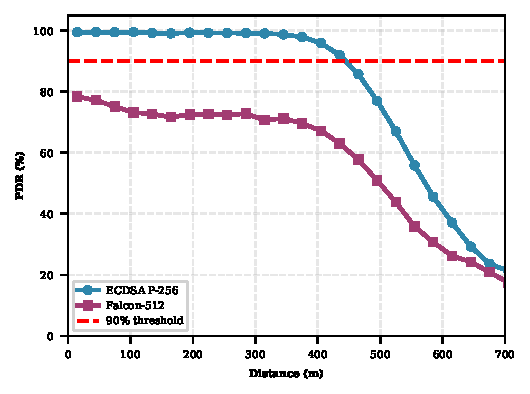
\includegraphics[width=\columnwidth]{figures/fig3_pdr_vs_distance.pdf}
\caption{PDR vs.\ distance for ECDSA P-256 and Falcon-512. The dashed line at 90\% denotes the safety-critical PDR threshold.}
\label{fig:pdr_dist}
\end{figure}

Figure~\ref{fig:pdr_dist} presents PDR as a function of transmitter-receiver distance. ECDSA maintains 100\% PDR at 0-400 m range and exhibits a gradual decline with increasing distance, remaining above the 90\% safety threshold~\cite{twardokus2025chasm} out to 400 to 450~m before dropping more sharply in the 500--700~m range. Falcon-512, by contrast, shows noticeably lower PDR even at close ranges below 100~m, where ECDSA is still 100\%. As distance increases, Falcon-512 also declines steeply, reaching substantially lower PDR in the 300--700~m range compared to ECDSA.

This early degradation at short distances indicates that the PDR penalty for Falcon-512 is not primarily driven by propagation loss, which would affect both algorithms similarly, but by channel contention. Falcon-512's 1,739-byte SPDU requires 4~subchannels at MCS~11, compared to 1~subchannel for ECDSA's 305-byte SPDU with MCS 7. This 4 times resource consumption with higher MCS increases collision probability even between nearby vehicles, with these effects becoming increasingly severe as distance grows.

\subsection{End-to-End Latency}

\begin{figure}[t]
\centering
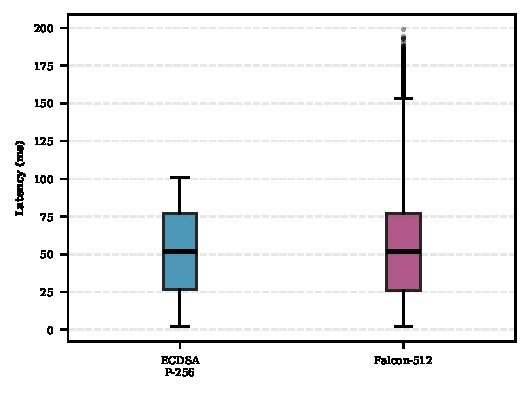
\includegraphics[width=\columnwidth]{figures/fig4_latency.pdf}
\caption{End-to-end latency distribution for ECDSA P-256 and Falcon-512). Box: Interquartile Range (IQR); whiskers:~1.5$\times$IQR; line:~median.}
\label{fig:latency}
\end{figure}

Figure~\ref{fig:latency} and Table~\ref{tab:results} present latency results. Mean latency is 51.92~ms for ECDSA and 51.82~ms for Falcon-512, a negligible 0.10~ms difference. The 95th percentile latencies are 96~ms (ECDSA) and 97~ms (Falcon-512). Both algorithms remain below the 100~ms SAE~J2945/1 safety threshold~\cite{sae_j29451}, confirming that Falcon-512's cryptographic operations impose negligible computational overhead. Latency is dominated by MAC-layer queuing and transmission delays, which remain comparable for both algorithms.

\begin{table}[t]
\centering
\caption{Performance Comparison (Scenario~C: 30~veh/km, LoS, $t \leq 200$~s)}
\label{tab:results}
\begin{tabular}{lcc}
\toprule
\textbf{Metric} & \textbf{ECDSA} & \textbf{Falcon-512} \\
\midrule
% Mean PDR$^{\dagger}$ (\%)    & 95.10 & 71.18 \\
% Median PDR$^{\dagger}$ (\%)  & 100.00 & 73.47 \\
Packet Size, Cert (B)         & 305   & 1,739 \\
Packet Size, Digest (B)       & 143   & 745   \\
Mean Latency (ms)             & 51.92 & 51.82 \\
95th Percentile Latency (ms)              & 96    & 97    \\
Mean PDR$^{\dagger}$ (\%)    & 95.10 & 71.18 \\
Verification Success (\%)     & 100   & 100   \\
\bottomrule
\multicolumn{3}{l}{\footnotesize $^{\dagger}$5GAA~P-190033 sliding-window method~\cite{5gaa_p190033}}
\end{tabular}
\end{table}

\section{Discussion}

These results demonstrate that Falcon-512 is \emph{computationally feasible} for C-V2X Mode~4 sidelink under moderate-high traffic conditions, but faces \emph{severe spectrum efficiency constraints} that significantly degrade PDR relative to ECDSA.

\textbf{Computational Viability:} The near-identical latency and 100\% verification success rate confirm that Falcon-512's cryptographic operations impose negligible computational overhead.

\textbf{Spectrum Efficiency Bottleneck:} The PDR degradation with 4.7 times packet size increase reveals that \emph{bandwidth consumption}, not computation, is the primary constraint. At moderate-high density (30~veh/km), the 4$\times$ subchannel requirement severely reduces channel capacity and increases collision probability. The 71.18\% mean PDR for Falcon-512 falls below the 90\% safety-critical threshold, indicating that direct ECDSA-to-Falcon migration is not viable at this density without mitigation.

\textbf{Mitigation Strategies:} Digest-based transmission reduces packet overhead but requires certificate pre-distribution via a Security Credential Management System (SCMS)~\cite{brecht2018scms}. Hybrid schemes (short-term ECDSA + long-term Falcon certificates) could balance quantum resistance with spectrum efficiency during migration periods.

\textbf{Deployment Implications:} Falcon-512 fits within SAE~J3161 transport block limits (MCS~11, 10~subchannels) without protocol modifications, satisfying a critical backward-compatibility requirement. However, the 71.18\% mean PDR at 30~veh/km demonstrates that direct deployment requires mitigation strategies, such as certificate segmentation or infrastructure-assisted distribution, to reach the safety-critical PDR threshold.

\section{Conclusion and Future Work}

% This paper evaluates Falcon-512 post-quantum signatures on C-V2X Mode~4 sidelink under moderate-high traffic density. Results show that while Falcon-512 is computationally viable, while the 4.7 times packet size overhead causes a 23.92~percentage point mean PDR degradation (95.10\% to 71.18\%), dropping Falcon-512 below the 90\% safety-critical threshold. These findings demonstrate that \emph{spectrum efficiency}, not computational cost, is the primary constraint for PQC adoption in bandwidth-limited V2X networks.

% Falcon-512 fits within SAE~J3161 transport block limits without protocol modifications, satisfying a critical backward-compatibility requirement. However, the 71.18\% mean PDR at 30~veh/km indicates that direct ECDSA-to-Falcon migration requires mitigation strategies such as digest-based certificates, hybrid cryptographic schemes, or infrastructure-assisted distribution.

% Future work will extend this evaluation to:
% \begin{itemize}
%     \item Additional traffic densities and NLOS propagation conditions
%     \item Additional PQC algorithms (Dilithium-2, hybrid ECDSA+Falcon schemes)
%     \item Density-aware algorithm selection guidelines and mitigation strategies
% \end{itemize}

% Comprehensive multi-algorithm, multi-scenario evaluation will inform quantum-resistant V2X security standardization and migration planning.

This paper evaluates Falcon-512 post-quantum signatures on C-V2X Mode~4 sidelink under moderate-high traffic density. Results show that while Falcon-512 is computationally viable, the 4.7 times packet size overhead causes a 23.92~percentage point mean PDR degradation (95.10\% to 71.18\%), dropping Falcon-512 well below the 90\% safety-critical threshold. Falcon-512 fits within SAE~J3161 transport block limits without protocol modifications, satisfying a critical backward-compatibility requirement. Nevertheless, these findings demonstrate that \emph{spectrum efficiency}, not computational cost, is the primary constraint for PQC adoption in bandwidth-limited V2X networks, and that direct ECDSA-to-Falcon migration at this density requires mitigation strategies such as digest-based certificates, hybrid cryptographic schemes, or infrastructure-assisted distribution.\\

Future work will extend this evaluation to additional traffic densities and NLOS propagation conditions to characterize how Falcon-512's PDR penalty scales with channel load and environment. Further studies will also incorporate additional PQC candidates, including Dilithium-2 and hybrid ECDSA+Falcon schemes, to enable comparative algorithm selection. Together, these efforts aim to develop density-aware deployment guidelines and inform quantum-resistant V2X security standardization and migration planning.

\section*{Acknowledgment}
This material is based upon the work supported by the National Center for Transportation Cybersecurity and Resiliency (TraCR) headquartered at Clemson University, Clemson, South Carolina, USA. Any opinions, findings, conclusions, and recommendations expressed in this material are those of the author(s) and do not necessarily reflect the views of TraCR, and the U.S. Government assumes no liability for the contents or use thereof.

\bibliographystyle{IEEEtran}
\bibliography{references}

\end{document}
